\documentclass[12pt,letterpaper]{article}

%Trennungsregeln etc.
\usepackage[english]{babel}

%Schriftart
%see http://www.tug.dk/FontCatalogue/ for more
%Ideen: baskervald
%for working: arev
\usepackage{baskervald}

%Sonderzeichenein-/ausgabe (http://tex.stackexchange.com/questions/44694/fontenc-vs-inputenc for questions)
\usepackage[utf8]{inputenc}
\usepackage[T1]{fontenc}

%Zeilenabstand, Optionen: singlespacing, onehalfspacing, doublespacing
\usepackage[onehalfspacing]{setspace}

%Seitenränder, hier oneside
\usepackage[left=2.5cm,right=2.5cm,top=2.5cm,bottom=2.5cm]{geometry}

%Anführungszeichen (for help see CTAN-package-page:  http://ftp.gwdg.de/pub/ctan/macros/latex/contrib/csquotes/csquotes.pdf)
\usepackage[strict=true,autostyle=true,german=quotes]{csquotes}

%Einrücklänge der ersten Zeile eines neuen Absatzes, standardmäßig drin
\setlength{\parindent}{1cm}

%Seitenzahlen
\usepackage{scrlayer-scrpage}
\pagestyle{scrheadings}
\ofoot[]{\pagemark}

%%Chapter/Section-Überschriften (Schriftart, Größe)
%Section-Überschriften
%\setkomafont{section}{\normalfont \bfseries \Large} 
%Inhaltsverzeichnis auch mit Serifen
%\setkomafont{disposition}{\normalcolor\bfseries}

%for pictures (png)
\usepackage{graphicx}

%insert hyperlinks
\usepackage[colorlinks=true, urlcolor=blue, linkcolor=black, citecolor = black]{hyperref}
\usepackage{url}

%Literaturverzeichnis
\usepackage[author year]{natbib}

%insert codesnippets
\usepackage{listings}
\usepackage{xcolor}
\definecolor{deepblue}{rgb}{0,0,0.5}
\definecolor{deepred}{rgb}{0.6,0,0}
\definecolor{deepgreen}{rgb}{0,0.5,0}
\lstset{ 
	language=Python, % choose the language of the code
	commentstyle=\itshape\color{yellow},
	basicstyle=\fontfamily{pcr}\selectfont\footnotesize\color{white},
	otherkeywords={self},
	keywordstyle=\color{violet}\bfseries, % style for keywords
	emph={MyClass,__init__},          % Custom highlighting
	emphstyle=\color{cyan},    % Custom highlighting style
	stringstyle=\color{deepgreen}
	numbers=none, % where to put the line-numbers
	numberstyle=\tiny, % the size of the fonts that are used for the line-numbers     
	backgroundcolor=\color{black},
	showspaces=false, % show spaces adding particular underscores
	showstringspaces=false, % underline spaces within strings
	showtabs=false, % show tabs within strings adding particular underscores
	frame=single, % adds a frame around the code
	tabsize=2, % sets default tabsize to 2 spaces
	rulesepcolor=\color{gray},
	rulecolor=\color{black},
	captionpos=b, % sets the caption-position to bottom
	breaklines=true, % sets automatic line breaking
	breakatwhitespace=false,
	stringstyle=\color{orange}
}


%Literaturverzeichnis
%\usepackage[author year]{natbib} %hier muss noch komme zwischen Autor und Jahr weg
%\documentclass{article}% use option titlepage to get the title on a page of its own.
\pagestyle{plain}
\usepackage{blindtext}
\title{Colorful Image Colorization with Tensorflow}
\date{\today}
\author{Sophia Schulze-Weddige \and Malin Spaniol \and Maren Born \\Implementing Artificial Neural Networks with Tensorflow \\Universität Osnabrück}
\begin{document}
\maketitle
\thispagestyle{empty}
\newpage
\thispagestyle{empty}
\tableofcontents
\newpage
\section{Introduction/Motivation}
Based on the paper \emph{Colorful Image Colorization} \citep{Zhang.2016} this project aims to reimplement a similar artificial neuronal net that transforms grayscale images into colorful pictures.\\
This involves first creating a dataset based on pictures that are converted into the CIELAB colorspace (Lab), such that the first channel \enquote{L} can be considered as input as it is grayscale whereas the \enquote{a} and \enquote{b} channel form the target labels to be predicted. Thus, the problem can be handled as classification task. In the second step, the aim was to closely rebuilt the layers of the original model (which used \enquote{caffe} \citep{jia2014caffe}) using tensorflow 2.0 (richtige version?).\\
Other project have trained convolutional neural networks (CNNs) on the color prediction problem before (e.g. \cite{Cheng_2015}, \cite{Dahl.2016}). The training data is easily available which enables training on large datasets. Problem about previous approaches is that they try to predict the ground truth rather than a possible truth. A conservative loss function tries to minimize Euclidean error between estimate and ground truth. As objects can have various plausible colors, these predictions are multimodal. Thus, the approach of Zhang et al. (2016) innovates a loss function that predicts plausible colors for pixels, rather than the original color \citep{Zhang.2016}.\\

\section{Important background knowledge (including reference to most relevant publications)}
Image colorization is for example made with photoshop. By colorizing old black and white pictures (\url{https://www.reddit.com/r/Colorization/}), images become more vivid and modern. The TV-series \emph{Greatest Events of WWII in Colour} (\url{https://www.imdb.com/title/tt9103932/}) used colorized footage in order to make the events more contemporary.\\
Automating the colorization problem with deep learning seems to be achievable, as training data is easy to get.\\

- what is CNN for image colorization?\\
In image classification, usually convolutional neural networks (CNNs) are used, which are inspired by the visual cortex of the brain. The idea is that highly specialized components or, in the case of CNNs, filters learn a very specific task, which is similar to the receptive fields of neurons in the visual cortex (QUELLE https://www.ncbi.nlm.nih.gov/pmc/articles/PMC1359523/ ). These components can then be combined to high-level features, which can then in turn be combined to objects that can be used for classification. In CNNs this concept is implemented by several successive convolutional layers in which one or more filters are slid over the input generating so-called feature maps. Each unit in one feature map looks for the same feature but in different locations of the input. In recent years, CNNs became so good that they outperform humans in many classification tasks (QUELLE http://karpathy.github.io/2014/09/02/what-i-learned-from-competing-against-a-convnet-on-imagenet/ , QUELLE https://arxiv.org/abs/1409.0575 ). Although machine learning exhibits very promising results and a lot of research and literature is available on the topic, many branches of industry still rely on traditional computer vision techniques in their implementation of image classification.\\

CNN apply trainable filtering kernels to extract features from an input image and project these features onto feature maps ~\citep{geron2019hands} ~\citep{bishop2006pattern} ~\citep{lecun1995convolutional}. Based on these maps, the label is predicted by a standard fully-connected layer.
Though using a CNN on the raw data images seemed promising, the results were only slightly better than chance level for the training accuracy.\\

- wie ist der status quo: -- related work\\
- was sind die schwierigkeiten von den colorization sache (sepia ding)\\
- was hat Zhang gemacht - was hat er besser gemacht\\

\begin{lstlisting}
#packages needed
import numpy as np 
import tensorflow as tf 
import cv2
from tensorflow.keras.preprocessing.image import ImageDataGenerator
from tensorflow.keras.models import Sequential
from tensorflow.keras.layers import Conv2D, MaxPooling2D, Flatten, Activation, BatchNormalization
	for loop
'ich bin ein string'
if
return
MyClass,__init__
\end{lstlisting}

%\section{``In-text'' listing highlighting}

- We started looking at this paper: \\
\url{https://arxiv.org/abs/1603.08511} , \\
- at their best solution
\section{The model and the experiment (MAIN PART). This part should feature code.}
As previously mentioned we re-implemented the main ideas from the paper by Zhang et al. This was done with two approaches, which are going to be explained in more detail in this chapter. In both approaches the ImageNet2012 dataset was used. Firstly, we implemented the model structure as described in the paper (see figure 1) and trained the model with the color layers of the input images as the target. Secondly, we translated the colorization task to a classification problem and trained the same model structure with the altered problem representation.\\
- hier nur erklären was wir machen\\
- Image colorization in general\\
- the model of the original paper\\
\begin{figure}[ht]
	\centering
	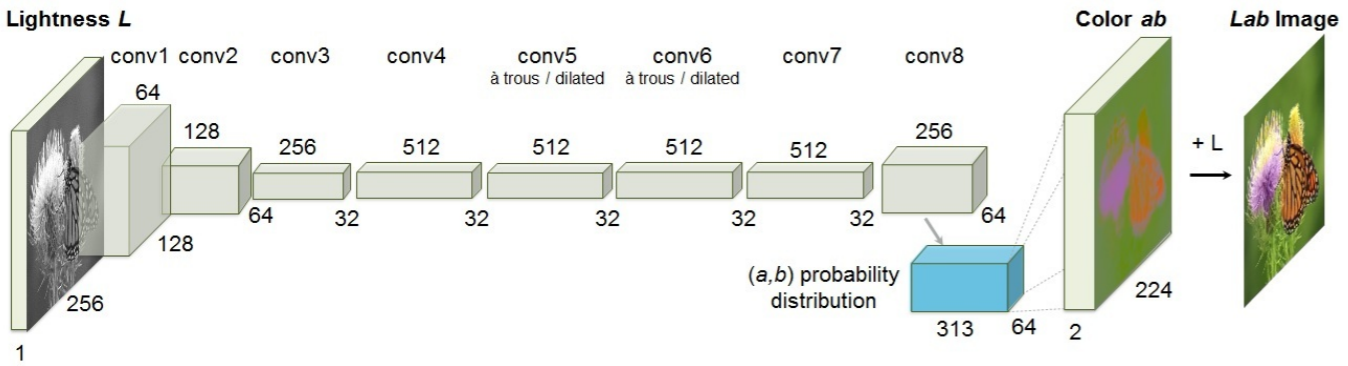
\includegraphics[width=1.0\textwidth]{layer.png}
	\caption{The network architecture of Zhang et al. (2016). }
	\label{fig1}
\end{figure}
- theoretical basis:\\

\subsection{Dataset}
To train our model we used images from the ImageNet2012 challenge, which were also used in the paper by Zhang et al. and which were available to us through the university server. As we were working with a large amount of data in each batch, it would have been impossible to load the whole dataset at once, hence we used a data generator to load the input and target images successively for each batch. Although there are inbuilt data generators available from keras that allow for some means of data augmentation, we built our costum generator to ensure the functionality we were aiming at. The generator takes the batch size and a list which contains the paths to the images that should be used. Besides the functionalities that one would expect, like shuffling after the whole training set has been seen, the generator further creates the input and target arrays as described in the following.
First, the images are loaded and resized to a uniform shape of (224, 224, 3), which corresponds to the height, the width and the number of the color channels, respectively. Then the images are transformed from BGR to LAB color space. The luminance layer (L layer) which displays most of the structure, is separated from the other two and used as the input for our model.  The remaining two layers (ab layers) encode the color information of the images and are used as the target of the model in the first approach. In the second approach, these first steps remain the same, but additionally the target arrays are transformed to match a classification task.\\
This is done in three main steps. The first step is to discretize the continuous color space and reduce the number of possible colors by quantizing the a and b color ranges into 11 bins. This yields a total of 121 possible colors by combining the a and b layers. In the second step, the a and b layers are combined into a single layer, which keeps the same height and width dimensions as before. This means the color information of each pixel is now encoded in a single number rather than two. Cantor pairing is used to generate a unique and deterministic number from the two a and b values of each pixel. As cantor pairing is reversible, one can easily translate the pairing result back to the original color values with no loss of information. Now that there is a single value for each pixel that encodes its color, the third and last step is to translate this value into a one-hot encoding. With the help of a dictionary, the cantor values are translated to the numbers from 0 to 120. These numbers then serve as the index in the one hot encoding. Hence, color values that were previously represented in two values (a and b color channels) are now encoded by the index within the one-hot encoding. The target array has a shape of (224, 224, 121) and at each pixel position lies a one hot vector.\\



- loading large amount of data\\
\url{https://machinelearningmastery.com/how-to-load-large-datasets-from-directories-for-deep-learning-with-keras/}\\
das ist \citep{Brownlee.2019}
\subsection{Preprocessing}
- image preprocessing documentation\\
\url{https://keras.io/preprocessing/image/#imagedatagenerator-class}\\
- preprocessing via ImageDataGenerator() from keras.prepeocessing.image\\
- takes in traindata, validation data and test data\\
- featurewise-center and featurewise std\\
- classmode: none -> is for predictions\\

\subsection{Modelstructure}
- besser hier layer und loss-function
\subsection{Layer}
- built the same layers aas Zhang et al, but no probability distribution\\
-networkstructure and design\\

\subsection{Loss-Function}
- the original loss-function\\
- we tried what loss function?\\
\section{Visualization and discussion of your results.}
oder lieber bilder als screenshot einfügen?\\
\begin{figure}[ht]
	\centering
	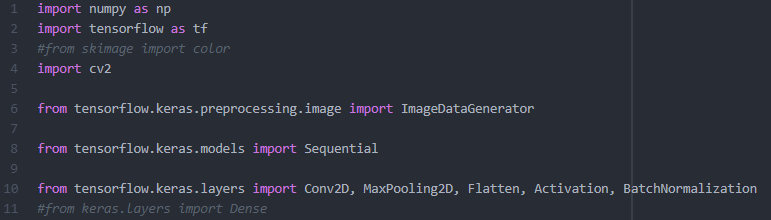
\includegraphics[width=1.0\textwidth]{bsp.png}
	\caption{Hier kann man dann auch noch etwas dazu schreiben}
	\label{bsp}
\end{figure}
%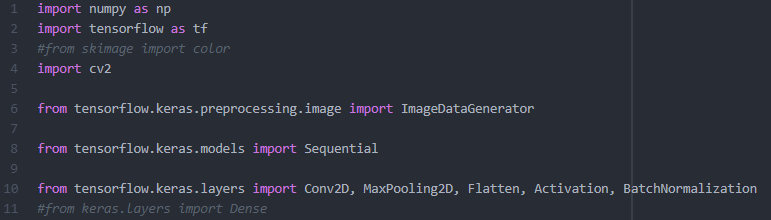
\includegraphics{bsp.png}
\subsection{Training}
\subsection{Testing}

\subsection{Conclusion and Future Work}
- vergleich ziehen zu Zhang\\

\section{Literature}
\label{Lit}
\bibliographystyle{apa}
\renewcommand{\bibsection}{}

\bibliography{lit}
	
\end{document}
